\chapter{Implementierung}\label{ch:Implementierung}

Dieses Kapitel wird sich der Implementierung der Thesis widmen. Es wird gezeigt, wie die Konzeption als Software umgesetzt wurde und einige wichtige Code-Stücke vorgestellt. Die Implementierung wurde auf dem ROS-Framework aufgebaut.

\section{Generelles zur Implementierung}
Die Implementierung baut auf Ubuntu LTS 16.04 mit der ROS-Version 'Lunar' auf, da diese beiden Komponenten das derzeit stabilste Duo bilden. Aufgrund mangelnder Kapazitäten, befindet sich das Ubuntu-System in einer Virtuellen Maschine, was, bis auf einen höheren Ressourcen-Verbrauch, allerdings keinerlei erkennbare Nachteile mit sich zog.

Generell ist das ROS-Framework in C++ und Python verfügbar, wobei diese Sprachen gemischt werden könnten, wenn sie auf verschiedenen Nodes genutzt werden. Als Programmiersprache wurde letztlich C++ verwendet, da es deutlich besser mit den verfügbaren Ressourcen umgeht. In den späteren Auswertungen hat sich diese Wahl positiv bestätigt, da 25 gleichzeitige Roboter eine Menge Ressourcen verschlungen haben und den verfügbaren Computer (auch wegen der VM) bereits an die Grenzen seiner Leistung brachte.

Da ein experimentelles Vorgehen direkt an realen Robotern zu Aufwändig wäre, insbesondere was die Zeitkosten für die Durchführung und Auswertung einer Simulation angeht, beruht die Implementierung auf der Node Turtlesim~\footnote{\url{http://wiki.ros.org/turtlesim}} von ROS~(siehe~\autoref{subsec:Grundlagen_Turtlesim}). Die Turtlesim wurde dahingehend angepasst, dass die Bilder der Turtles durch wesentlich kleinere Bilder schwarzer Pfeile ersetzt wurden die visuellen Aufschluss auf Position und Aurichtung erlauben. Dadurch wurde mehr Platz und Übersichtlichkeit gescahffen. Das Verhalten der Turtles selbst in der Simulation ist unverändert.

Generell ist die Turtlesim nicht dafür gemacht worden, aufwändigere Simulationen zu erproben. Der Zweck ist es einen einfachen Einstieg in das ROS-Framework zu geben und Neulinge durch die Tutorials zu begleiten. Sie bietet aber eine grafische Oberfläche, die bei der Implementierung sehr nützlich ist, insbesondere um Fehler besser entdecken zu können.
Bei der Implementierung wurde viel Wert auf eine modulare Bauweise gesetzt. Die Bewegungsbefehle die aktuell an die Turtlesim gehen sind abstrahiert und lassen sich später schnell auf das System des jeweiligen Roboters umschreiben. Andere Nachrichten gehen nicht über die Turtlesim, wodurch die Bewegung das einzige Sub-System ist, dass es nachher anzupassen gilt.

\section{Nachbau des Schwarms nach Craig Reynolds}

\begin{wrapfigure}{r}{\pictureWidth}
	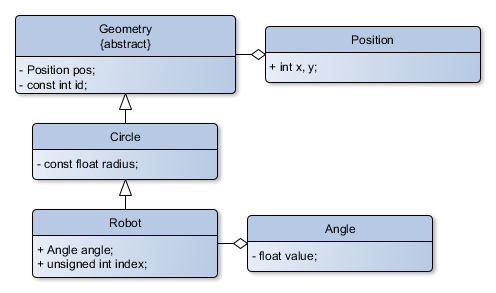
\includegraphics[width=\pictureWidth,keepaspectratio]{graphics/Klassendiagramme/KlassendiagrammRobot.png}
	\caption{Die Klassenhierarchie eines Roboter-Objektes}
	\label{pic:KlassendiagramRoboter}
\end{wrapfigure}

Sendet man einen Bewegungs-Befehl an die Turtlesim, wird diese den Befehl für 1 Sekunde ausführen und nach Abschluss die Position des Roboters automatisch an die Subscriber verteilen. Die Subscriber erhalten in ROS ihre Informationen immer über Callback-Funktionen. Da diese Funktionen statisch sein müssen, ist es nicht einfach möglich die Daten in einem Objekt zu speichern, sondern sie müssen in globalen Variablen untergebracht werden.
Die Informationen über die Position der Roboter werden in einem Array gespeichert. Da die Roboter IDs haben, ist es leicht diese bei 0 beginnen zu lassen und sie dann als Index zur Adressierung innerhalb des Arrays zu nutzen.

Da Roboter eine Position und eine Fläche haben die deren Körper darstellt, macht es am meisten Sinn ihnen einen Kreis als geometrische Form zu vererben, sodass letztlich die Klassen-Struktur aus \autoref{pic:KlassendiagramRoboter} entsteht (Funktionen wurden ausgelassen). Der Nutzen der Klasse \highlight{Angle} ist der, dass die Klasse automatisch darauf achtet im Bereich [0, 360] zu bleiben: \highlight{Angle(350) + Angle(20) == Angle(10)}.

\subsection*{Messages}

Die Steuerung der Roboter innerhalb der Turtlesim geschieht nicht direkt durch das eigene Programm. Stattdessen müssen Nachrichten an die Turtlesim gesendet werden die dann letztlich die Roboter bewegt. Insgesamt werden dafür 5 Nachrichten verwendet. Die Nachrichten-Typen werden der Übersichtlichkeit halber in einer verkürzten Schreibweise vorgestellt, wie sie in ROS nicht erlaubt, von Programmiersprachen wie C++ oder Java, aber bekannt ist. Einige Nachrichten arbeiten mit dem Topic 'turtleX', was nichts anderes bedeutet als eine ID für die Roboter der Turtlesim (turtle1, turtle2, ...).

\begin{lstlisting}[style=ros, title=turtlesim/Pose.msg]
	// Empfangen von dem Topic: turtleX/pose
	// Gibt Feedback zur Position und Ausrichtung des Roboters
	// Wird in dieser Arbeit genutzt, um die Position der Roboter zu speichern
	float32 x, y, theta, linear_velocity, angular_velocity
\end{lstlisting}

\begin{lstlisting}[style=ros, title=geometry\_msgs/Twist.msg]
	// Gesendet an das Topic: turtleX/cmd_vel
	// Fahrbefehl fuer den Roboter, wird 1 Sekunde lang ausgefuehrt
	// Wird in dieser Arbeit genutzt, um die Roboer geradeaus zu fahren zu lassen
	Vector3  linear, angular
\end{lstlisting}

\begin{lstlisting}[style=ros, title=turtlesim/TeleportRelative Service]
	// Gesendet an den Service: turtleX/teleport_relative
	// Teleportiert den Roboter zu einem relativen Ort
	// Wird in dieser Arbeit genutzt, um die Roboter vor dem Fahrbefehl zu drehen
	float32 linear, angular
	---
\end{lstlisting}

\begin{lstlisting}[style=ros, title=turtlesim/Spawn Service]
	// Gesendet an den Service: spawn
	// Erschafft einen neuen Roboter in der Turtlesim
	float32 x, y, theta
	string name
	---
	string name
\end{lstlisting}

\begin{lstlisting}[style=ros, title=turtlesim/SetPen Service]
	// Gesendet an den Service: turtleX/set_pen
	// Schaltet den Pen aus. Ein 'Stift' der den gefahrenen Weg markiert
	uint8 r, g, b, width, off
	---
\end{lstlisting}

\subsection*{System-Takt: Ticks}

Der Ablauf eines Programms geschieht in Ticks (der Takt des Systems, periodische Zeitabstände), in denen zuerst eine Aktion gestartet und danach eine kurze Zeit gewartet wird um Nachrichten anderer Roboter zu empfangen und zu verarbeiten. Es ist damit impliziet nur eine Bewegungs-Aktion pro Tick möglich. Diese kann allerdings Drehung und Fahren kombinieren.
Die Bewegung einer Turtle wird von ROS genau 1 Sekunde lang ausgeführt. Die Steuerung der bewegten Entfernung pro Tick lässt sich daher nur über die Geschwindigkeit der Bewegung steuern. In der Praxis hat sich aufgrund von weiteren Verzögerungen in der Turtlesim eine Tick-Länge von 1.1 Sekunden bewährt.

Entschließt sich ein Roboter dazu sich nicht zu bewegen, muss er einen 'leeren' Bewegungsbefehl senden, der dazu führt, dass sich der Roboter nicht bewegt und somit einen Tick abschließen, statt einfach zu warten und nichts zu senden. Der Grund hierführ liegt darin, dass die Systeme Single-Thread Architekturen sind und das Abfragen der Topics expliziet ausgelöst werden muss. Dies geschieht über eine Funktion in ROS, die aufgerufen wird und die automatisch alle abonnierten Topics abfragt, um dann die entsprechenden Callback-Funktionen auszuführen. Außerdem werden dadurch die eigenen Daten auf den Robotern aufgefrischt und eventuelle Informationen gesendet, die nichts mit der Bewegung zu tun haben. Das abschließen eines Ticks synchronisiert somit generell die Daten des eigenen Systems mit dem der anderen.

Die Ticks sind trotz allem keine globalen Ticks, die jeden Roboter gleichzeitig. Jeder Roboter arbeitet auf seiner Zeitlinie und agiert unabhängig der Ticks der anderen Einheiten.

\subsection*{Einhalten der 4 Grundregeln}
Die Roboter wurden als autonome Einheiten konzipiert die sich ausschließlich anhand von 3 fixen Parametern bewegen und dabei versuchen die 4 Grundlegen des Schwarmverhalten einzuhalten. Grundsätzlich werden von einem Roboter nur andere Einheiten beachtet, die in einem gewissen Radius um ihn herum positioniert sind. Daher wird Am Anfang eine Liste derjenigen erstellt. Dies geschieht durch simples iterieren über die Liste aller Roboter und einer Berechnung über Pythagoras.

\subsubsection*{Ausrichtung: Passe deine Bewegungsrichtung deinen Nachbarn an}

\begin{wrapfigure}{r}{\pictureWidth}
	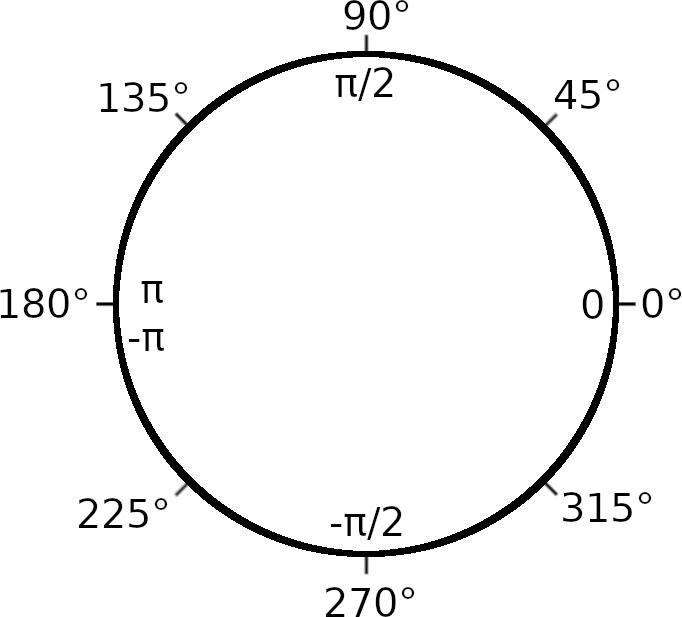
\includegraphics[width=\pictureWidth,keepaspectratio]{graphics/WinkelTemplate.png}
	\caption{Winkel-Übersicht}
	\label{pic:WinkelUebersicht}
\end{wrapfigure}

ROS selbst arbeitet bei Winkeln mit dem Bereich von [-3.14, 3.14], wohingegen die Steuerung der Roboter mit dem Bereich [0°, 360°] arbeitet, da dieser besser bearbeitet (und von Menschen gelesen) werden kann. Außerdem ist dadurch generell eine Abstraktions-Ebene entstanden die es später erlaubt mit jedem bliebig anderen Winkel-System zu arbeiten.
Eintreffende Positionsdaten, von anderen Robotern, müssen also erst in die interne Darstellung umberechnet werden. Ebenso wird der Winkel vor dem Senden eines Bewegungs-Befehls automatisch so umberechnet dass ROS ihn akzeptiert. Wird ROS ein zu großer Winkel gesendet, z.B.: 5, so wird sich der Roboter einfach sehr schnell drehen und wärend dieser Zeit schwer unkontrollierbar sein, sonst aber keine weiteren Fehler produzieren.
In~\autoref{pic:WinkelUebersicht} ist eine Übersicht über die Winkel zu sehen wie sie im System und von ROS genutzt werden.
 
\subsubsection*{Zusammenhang: Versuche deinen Nachbarn nahe zu sein}

Für die Berechnung des Mittelpunkts der Nachbarschaft, wurde schlicht die Liste der Roboter, die nahe genug sind, genommen und ein mathematischer Durchschnitt gebildet. Die Koordinaten wurden danach von den eigenen Abgezogen und die resultierenden X/Y-Werte als Vektoren genutzt um den Winkel zu berechnen, den der Mittelpunkt zum Roboter hat. Anschließend wurde noch die Different dieses Winkels zu dem Winkel gebildet, den man fahren wollte. Ein prozentualer Wert dieser Differenz wurde dann vom Winkel abegzogen.

\subsubsection*{Abschottung: Vermeide Kollisionen mit deinen Nachbarn}

Um Kollisionen mit anderen Robotern zu vermeiden, werden zur Kollisionserkennung interne Simulationen verwendet. Im Grunde bedeutet dies, dass berechnet wird wo der Roboter mit dem aktuell gewünschten Winkel und normaler Geschwindigkeit hinfahren wird. Ist dieser Ort weit genug von anderen Robotern entfernt, wird er akzeptiert. Ist er es nicht, wird der gewünschte Winkel in Schritten von 1° erst nach links und dann nach rechts verändert und erneut geschaut ob es am Zielort zu einer Kollision kommen wird.

\paragraph*{Unzureichende Erkennung auf dem Weg}
Um die Berechnung einfacher zu gestalten und Ressourcen zu schonen wurde nicht der Weg selbst überprüft. Es ist also möglich, dass ein Roboter weder auf seinem Ursprungs- oder Zielort mit anderen Robotern kollidiert, wohl aber auf dem Weg dorthin. Ebenfalls ist es in der Turtlesim nicht möglich, eine angefangene Bewegung wieder abzubrechen. Kommt es also während der Ausführung zu einer Kollision, z.B. weil sich zwei Roboter aufeinander zubewegen, kann diese nicht mehr verhindert werden. Ein Ausgleich in der Simulation ist durch eine Abfrage gegeben, ob sich zwei Roboter 'ineinander' befinden. Die entsprechenden Roboter werden dann auf direkter Luftlinie voneinander weggeschoben, um wieder einen plausiblen physikalischen Zustand einzunehmen.

Im der Praxis sollte eine Kollision auf dem Weg kein Problem darstellen, da mit parallelen Threads nebenläufiges Verhalten ingesetzt werden kann. Es wäre also ohne weiteres möglich zu fahren und gleichzeitig die Positionen der anderen im Auge zu behalten. Außerdem ließe sich, im Falle einer Single-Thread-Architektur, die Frequenz der Ticks wesentlich schneller eingestellen, sodass sich die Roboter effektiv nur wenige Millimeter pro Tick bewegen, dafür aber mit über 100 Ticks pro Sekunde. Letztlich kommt es auf die Leistung des verwendeten Computers an.

\subsubsection*{Flucht: Fliehe vor Dingen, die eine potentielle Gefahr darstellen}

\begin{wrapfigure}{r}{\pictureWidth}
	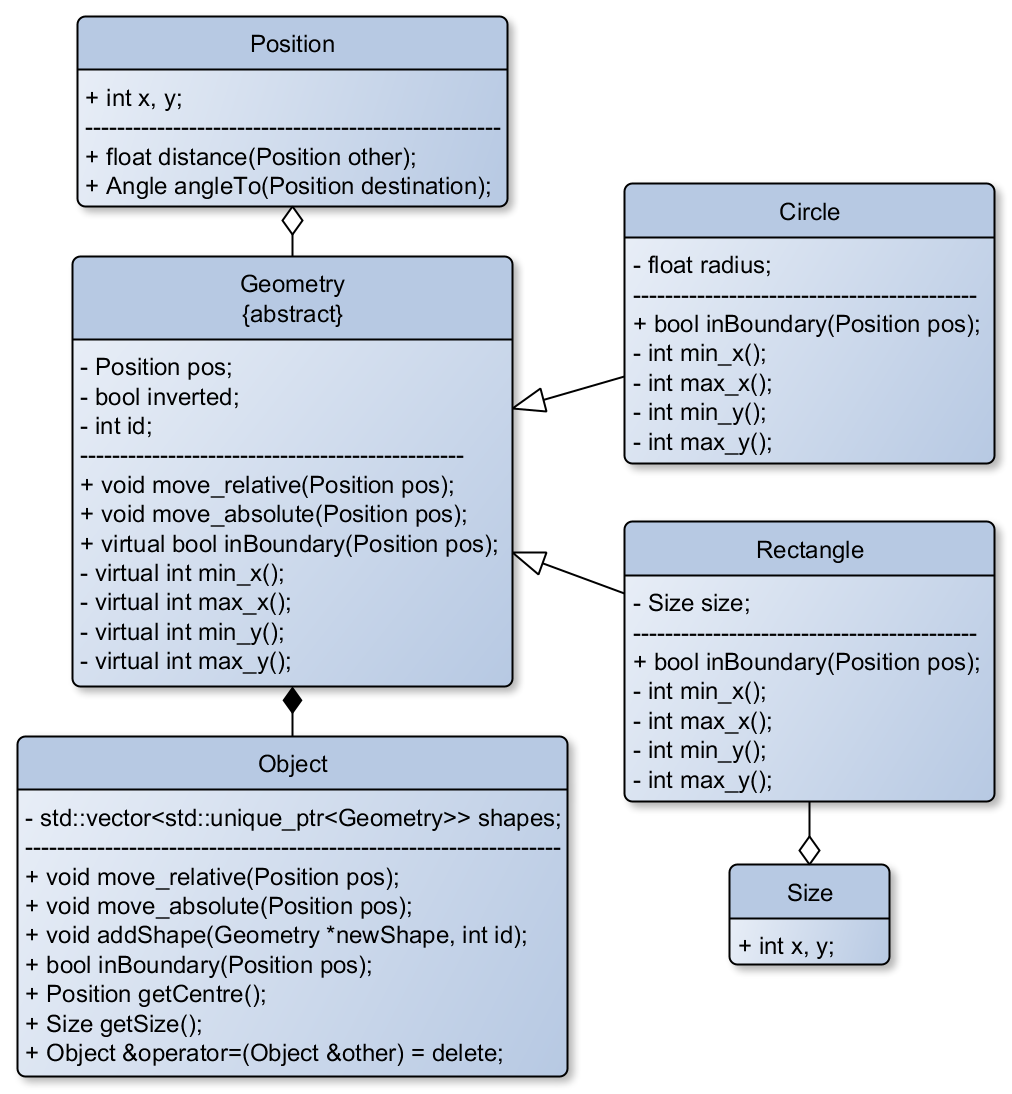
\includegraphics[width=\pictureWidth,keepaspectratio]{graphics/Klassendiagramme/KlassendiagrammObject.png}
	\caption{Die Klassenhierarchie eines Hindernisses}
	\label{pic:KlassendiagramObjekt}
\end{wrapfigure}

Kollisionen mit Gefahrenzonen werden genau wie Kollisionen mit Robotern erkannt und verhindert.
Um Gefahrenzonen darzustellen, wird auf Abstraktion und Vererbung gesetzt. Es gibt, wie in \autoref{pic:KlassendiagramObjekt} zu sehen ist, eine Hierarchie von Klassen aus denen sich die Zonen zusammensetzen lassen. Die \highlight{Geometry}-Klassen die sich in der \highlight{Object}-Klasse befinden werden alle von dieser gesteuert. Bewegt sich das Objekt, bewegen sich alle darin enthaltenen Geometrien. Das Hinderniss bleibt dadurch immer in einem plausiblen Zustand. Ebenfalls muss nur die \highlight{Object}-Klasse nach einer Kollision befragt werden, diese leitet die Anfrage an alle Geometrien weiter.


\subsection*{Berechnung der Bewegung}

Die Berechnung der Bewegung geschieht letztlich in den Schritten die in \autoref{pic:AblaufSchwarm} gezeigt werden.

\begin{wrapfigure}{r}{\pictureWidth}
	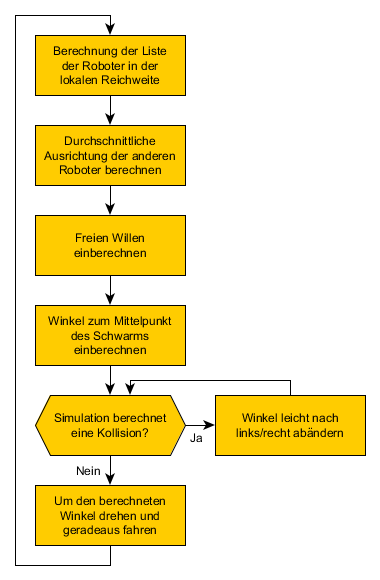
\includegraphics[width=\pictureWidth,keepaspectratio]{graphics/ImplSchwarm.png}
	\caption{Ablaufdiagramm Schwarm}
	\label{pic:AblaufSchwarm}
\end{wrapfigure}

%\begin{enumerate}
%\item Berechnung der Liste der Roboter, die sich innerhalb der lokalen Reichweite befinden
%\item Durchschnittliche Ausrichtung der nahen Roboter berechnen. Ergebniss in \highlight{ZielWinkel}
%\item Zufallsentscheidung über den freien Willen im Bereich [-x/2, x/2]. Ergebniss auf \highlight{ZielWinkel} aufrechnen
%\item Winkel zum Mittelpunkt des eigenen Schwarmes aus- und aufrechnen nach \highlight{ZielWinkel -= (Mittelpunkt - Zielwinkel) * x\%}
%\item Mit berechnetem Winkel Simulation durchführen um Kollisionen zu erkennen. Gegebenenfalls Winkel und Geschwindigkeit nachbessern
%\item Um den berechneten Winkel drehen und mit berechneter Geschwindigkeit geradeaus fahren
%\end{enumerate}









\section{Anführer}

Da der Anführer seinen Schwarm lenkt, verfällt die Einheit, die zum Anführer wurde, in ein spezielles Verhalten. Dieses Verhalten hat mit der bisherigen Implementierung wenig zu tun. Auf das Ziel zuzusteuern und den Schwarm dabei nicht zu verlieren, ihn sogar wieder einzufangen, wenn er abhanden kommt, kann mit den bisherigen Schwarmregeln nicht umgesetzt werden. Aus diesem Grund ist die Implementierung weniger ein umändern der bisherigen Implementierung, sondern es wird eher ein neues Verhalten hinzugefügt und eine Abzweigung im Code um dieses auszuführen.

\subsection*{Generelles Verhalten}

Der Anführer ist ein Zweig im normalen Verhalten der Roboter. Erhält ein Roboter eine Nachricht vom Typ \highlight{New\_Mission}, richtet er sich nach diesem Ziel aus und fährt ihm entgegen. Behindert ein anderer Roboter, dass der Anführer geradeaus weiter kann, verringert er seine Geschwindigkeit oder bleibt letztlich 1 Tick lang stehen. Ist er nahe genug am Ziel angekommen, fällt er in sein altes Verhalten zurück.
\autoref{pic:AblaufAnführer} zeigt das Verhalten wie es umgesetzt wurde.

\begin{wrapfigure}{r}{\pictureWidth}
	\includegraphics[width=\pictureWidth,keepaspectratio]{graphics/ImplAnführer.png}
	\caption{Ablaufdiagramm Schwarm}
	\label{pic:AblaufAnführer}
\end{wrapfigure}

\subsection*{Einbindung des Anführers in ROS}

Die Einbindung der Anführer in ROS geschah mit einem zusätzlichen Subscriber der das Topic \highlight{flock/mission/new} abonniert hat. Die Funktion des entsprechenden Callbacks nimmt die \highlight{New\_Mission} an und speichert sie, wenn die ID in der Mission der ID des Roboters entspricht, in einer globalen FIFO-Struktur. Ein Roboter überprüft diese Struktur in seinem normalen Ablauf immer wieder und arbeitet die Mission ab, wenn er eine findet.
Da die Implementierung als Single-Thread-Architektur implementiert ist, braucht es auch keine entsprechenden Vorsichtsmaßnahmen, wie sie bei Multi-Thread üblich sind.
Die Struktur der Nachricht konnte für die Implementierung so beibehalten werden, wie sie in der Konzeption vorgegeben wurde.

\begin{lstlisting}[style=ros, title=Nachrichten-Typ: New\_Mission]
	uint8	leader_id	// Die ID des ausgewaehlten Anfuehrers
	float32 pos_x		// Position des Ziels entlang der X-Achse
	float32 pos_y		// Position des Ziels entlang der Y-Achse
\end{lstlisting}



% ================================================================================================================
% ================================================================================================================
% ================================================================================================================


\section{Transport von Waren mit Hilfe eines Schwarms}

Das letztliche Ziel dieser Arbeit ist es zu prüfen, ob es möglich, und sinnvoll, ist Gegenstände mit Hilfe eines autonomen Schwarms zu transportieren. Dazu musste der Schwarm nun dazu gebracht werden Waren zu bewegen ohne die einzelnen Roboter zu sehr zu beeinflussen. Da generell die Roboter nicht zentral gesteuert werden sollen und auch die Logik möglichst simple bleiben soll, sollte das Programm der einzelnen Einheiten möglichst wenig verändert werden und der 'natürliche' Trieb der Einheiten genutzt werden.

\subsection*{Erteilen von Aufträgen}

Eine der ersten Dinge im Ablauf eines Transports ist die Erteilung des Auftrags. Dazu wurde ein neuer Nachrichten-Typ Namens 'MissionNew' im ROS-Netzwerk eingeführt der die folgenden Felder hat:

\begin{lstlisting}[frame=L]
uint8 robot_index_from
uint8 robot_index_to

uint8 leader_number
uint8 mission_id

float32 object_position_x
float32 object_position_y

float32 object_size_x
float32 object_size_y

float32 target_x
float32 target_y
\end{lstlisting}

Der Nachrichten-Typ definiert eine Spanne von Robotern die den Auftrag ausführen sollen. Diese werden mit ihren IDs angesprochen. Das Intervall der IDs ist, gemäß Programmierstandards, als halboffenes Intervall definiert: [robot\_index\_from, robot\_index\_to[.
leader\_number gibt die Anzahl der Leader an die verwendet werden sollen und mission\_id gibt dem derzeitigen Auftrag eine fixe ID um diesen und zugehörige Dinge genau identifizieren und verbinden zu können.
Mit object\_position\_x/-\_y ist die Startposition des zu transportierenden Objektes angegeben. Zusammen mit object\_size\_x/-\_y, welche die Ausmaße des Objektes angeben. Die Position des Objekts ist als Mitte des Objekts definiert.
target\_x/-\_y gibt die letztliche Position an die das Objekt einnehmen soll.

Der Auftrag wird von außen an das Topic 'flock/mission/new' gesendet. Der Ersteller des Auftrags muss keine ROS-Node sein, auch wenn dies verschiedene Vorteile hätte. Dadurch das ROS-Topics auch über das Terminal engesprochen werden können, ist das Senden der Nachrichten auch über jedes andere Programm möglich. Das Topic für die neuen Missionen wird von jedem aktiven Roboter abonniert. Entsprechend nimmt jeder Roboter Notiz von diesem Auftrag, auch wenn er nicht direkt mit seiner ID angesprochen wird.

\subsection*{Von Gefahrenzonen zu Sicherheitszonen}

Um die betreffenden Roboter in die Zone zu senden, auf der ihnen später das Transportobjekt aufgesetzt wird, wird ein Mechanismus verwendet der bereits vorher Einzug in das ROS-System hielt: Gefahrenzonen. Diese wurden leicht angepasst um sie invertieren zu können und somit aus einer Gefahrenzone eine Sicherheitszone zu machen. Ist ein Bereich als Sicherheitszone definiert, ist jeder andere Bereich automatisch eine Gefahrenzone.
Dieser Mechanismus birgt nur eine kleine Änderung im System, schafft es aber Roboter in einen bestimmten Bereich zu locken ohne sie aktiv steuern zu mpsse, indem einfach ihr 'natürlicher' Trieb verwendet wird, von Gefahren zu flüchten.

Wird ein Auftrag erteilt, so nehmen die Roboter die dem Auftrag zugeteilt sind, eine neue Sicherheitszone auf, die den Ausmaßen und der Position des Transportobjekts am Aufnahmeort entsprechen. Roboter die nicht dem Transport zugeteilt wurden, werden diese neue Zone als Gefahrenzone auffassen und versuchen sich diesem Gebiet fernzuhalten.

Ein Objekt kann grundsätzlich aus verschiedenen Geometrien zusammengesetzt werden. Dadurch ist es möglich nicht nur Objekte zu transportieren die eine einfache Form wie Rechtecke oder Kreise haben, sondern verschiedene Rechtecke können dann zu einem 'L' oder 'U' zusammengesetzt werden.

\begin{wrapfigure}{r}{\pictureWidth}
	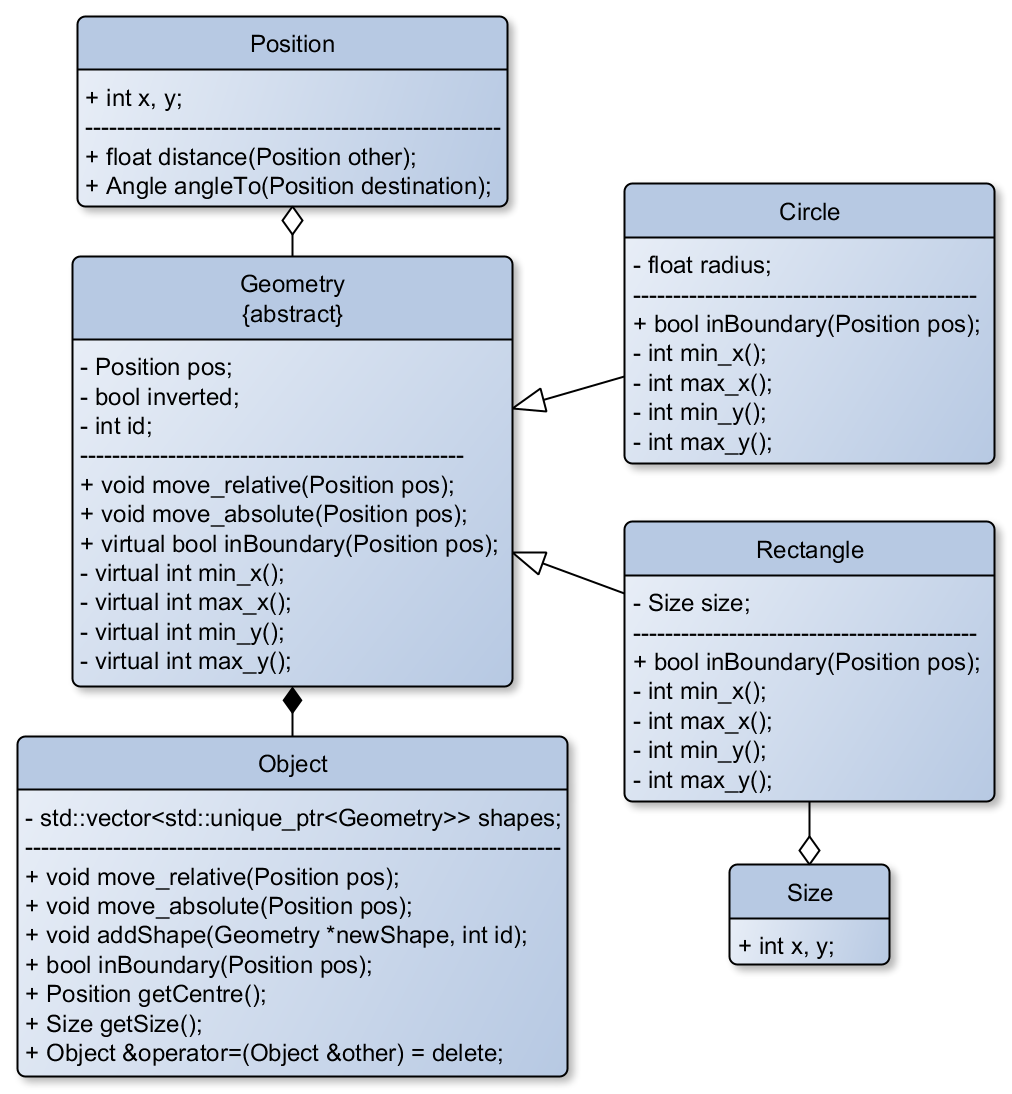
\includegraphics[width=\pictureWidth,keepaspectratio]{graphics/Klassendiagramme/KlassendiagrammObject.png}
	\caption{Die Klassenhierarchie des Objekt-Systems}
	\label{pic:KlassendiagrammObject}
\end{wrapfigure}

\paragraph*{Implementierung}
Die Klassenhierarchie ist wie in \autoref{pic:KlassendiagrammObject} dargestellt. Die Implementierung eines Objekts ist als Sammelklasse definiert, die verschiedene Geometrien unter sich vereint. Die Geometrien haben eine Hauptklasse von der sie sich ableiten. Die abgeleiteten Klassen müssen letztlich nur noch definieren, wann etwas innerhalb ihrer Fläche ist und was ihre Ausmaße im zweidimensionalen Raum sind. Wird ein Objekt auf eventuelle Kollisionen abgefragt, muss dieses letztlich nur noch über die inneliegenden Geometrien iterieren und sobald eine Kollision statt fand ist das Gesamtergebnis ebenfalls eine Kollision.

\subsection*{Füllen eines Raums}

Wird eine Sicherheitszone definiert, versuchen die Roboter, die sich in der Gefahrenzone befinden, auf möglichst schnellstem Wege die Sicherheitszone zu betreten. Dazu wird das Zentrum der Sicherheitszone ins Ziel genommen und (ohne mit anderen Robotern zu kollidieren) der direkte Weg darauf zu genommen. Dabei kann es dann allerdings vorkommen, dass eine komplexere Form nicht vernünftig gefüllt werden kann, oder dies sehr lange dauert. Da ein eintreffender Roboter so lange auf den Mittelpunkt zufahren würde, bis die Roboter darin sich genug verteilt haben um genug Platz für den neuen Roboter zu schaffen.

Ein Algorithmus wie man es schafft mit Roboter einen definierten Raum zu füllen lässt sich in (\note{HIER; QUELLE}) finden. Dieser Algorithmus lässt sich aufgrund anderer Fähigkeiten bei den Robotern nicht und dem gewünschten Schwarmverhalten nicht vollständig nachbilden. Eine andere, bereits implementierte Fähigkeit, lässt sich dagegen gut nutzen um den Algorithmus annähernd nachzubauen: Ausweichen.

\begin{wrapfigure}{r}{\pictureWidth}
	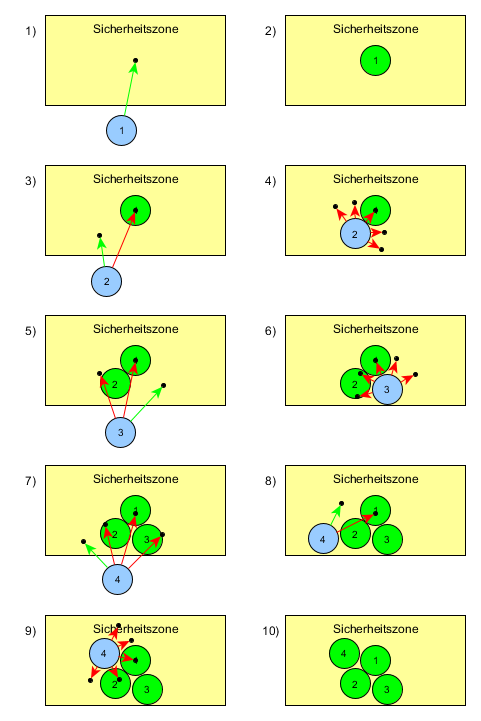
\includegraphics[width=\pictureWidth,keepaspectratio]{graphics/AlgorithmusAusweichenTransport.png}
	\caption{Roboter füllen das Transportobjekt}
	\label{pic:AlgorithmusAusweichenObjekt}
\end{wrapfigure}

Betritt ein Roboter die Sicherheitszone des Transport-Objekts, reduziert dieser seine Geschwindigkeit und fährt langsam weiter auf den Mittelpunkt zu. Neu ankommende Roboter werden durch die vorderen, viel langsameren Roboter zum Ausweichen gezwungen, was letztlich dazu führt, dass die Roboter sich seitlich verteilen, aber langfristig den Nachfolgern Platz machen. Ist ein Roboter nahe genug am Mittelpunkt angekommen oder findet in einem Umkreis von [-90°, 90°] keinen Platz mehr der näher am Mittelpunkt ist als der aktuelle, bleibt er stehen. Roboter die stehen bleiben senden den anderen Robotern ihres Schwarms ein entsprechendes Signal dass sie bereit sind. Haben alle Roboter erkannt dass die anderen bereit sind, ist die Phase des Eintreffens am Abnahmepunkt abgeschlossen.

Von hier an braucht es ein Event dass den Robotern zeigt dass sie mit dem Transportobjekt Richtung Ziel losfahren können. Möglich wäre eine Zeitsteuerung für streng automatisierte Prozesse. Aber auch interne Signale über ROS sind möglich. Durch die ID die jeder Auftrag hat, wäre eine einfache Nachricht '[TransportID\#][Losfahren]' bereits zielführend.

\paragraph*{Der Algorithmus am Beispiel}
\autoref{pic:AlgorithmusAusweichenObjekt} zeigt den Algorithmus anhand eines Beispiels mit 4 Robotern.

Der erste Roboter versucht zur Mitte des Objekts zu gelangen und findet sofort Zugang zum Objekt. Er reduziert seine Geschwindkeit und platziert sich langsam im Mittelpunkt des Objektes. Da seine Nähe zum Mittelpunkt klein genug ist, bleibt er letztlich stehen.

Der nächste Roboter kommt, wird allerdings von seinem Vorgänger leicht blockiert. Das führt dazu dass dieser versucht nach links auszuweichen und damit Erfolg hat. Er betritt die Zone, findet aber keinen besseren Ort und bleibt daraufhin stehen.

Der dritte Roboter wird ebenfalls von seinen Vorgängern blockiert, findet aber rechts eine Stelle. Nachdem er diese eingenommen hat findet auch er keine bessere Stelle und bleibt ebenfalls stehen.

Der vierte Roboter findet zunächst links eine Stelle und betritt daraufhin die Zone. Er verlangsamt seine Bewegung und sucht nun nach Stellen die ihn ohne Kollisionen näher zu seinem Ziel führen, wobei er einmal Roboter\#2 umkreist. In der Lücke zwischen Roboter\#2 und Roboter\#1 findet er die beste Stelle und bleibt dort anschließend stehen. Der Algorithmus für diese 4 Roboter ist damit abgeschlossen. Sie stehen alle in der Fläche des Transportobjektes und stehen still, bereit die Lieferung entgegen zu nehmen.

\subsection*{Der Transport}

Um den Transport selbst zu realisieren bedient man sich der Hilfe der Anführer. Diese richten sich dynamisch nach dem Winkel aus, den das Transportobjekt zum Ziel hat, wie \autoref{pic:AlgorithmusTransport} zeigt. Danach fangen sie an sich langsam in die Richtung zu bewegen in die sie sich ausgerichtet haben. Die anderen Roboter werden sich aufgrund des Gruppenverhaltens ebenfalls mehr oder weniger nach ihren Anführern ausrichten und das Objekt so langsam Richtung Ziel bewegen.

\begin{wrapfigure}{r}{\pictureWidth}
	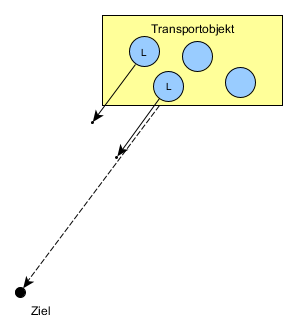
\includegraphics[width=\pictureWidth,keepaspectratio]{graphics/AlgorithmusTransport.png}
	\caption{Der Transport des Objekts}
	\label{pic:AlgorithmusTransport}
\end{wrapfigure}

\subsubsection*{Einhalten der Richtung hat Priorität}
Kann ein Anführer keine normale Bewegung ausführen, weil er sonst mit einem anderen Roboter kollidieren würde, darf er nicht versuchen auszuweichen, da dies sonst die Ausrichtung der passiven Roboter negativ beeinflussen könnte. Stattdessen drosselt er zunächst sein Bewegungstempo oder bleibt, falls notwendig, ganz stehen. Die richtige Richtung beizuhalten ist wichtig, da sich passive Roboter nicht unmittelbar nach ihren Anführern ausrichten. Gerade wenn es zahlenmäßig wenige Anführer im Vergleich zu passiven Robotern sind, kann es einige Zeit dauern, bis die Einheiten so weit beeinflusst wurden, dass sie in die gewünschte Richtung zeigen. Dreht sich ein Anführer in die verkehrte Richtung, vielleicht sogar in die entgegengesetzte, kann dies zu einer Kettenreaktion führen die alle Roboter betrifft und zusätzlich das Transportobjekt stark vom Weg abbringen.

\subsubsection*{Abschluss des Transports}






